\section*{Method}
\label{Method}
The subjects were shown pictures of each set of speakers as they appear in \autoref{fig:speakers}. They were then asked to rate their attributes on a VAS with 16 bipolar word-pairs. 

\begin{figure}[H]
\centering
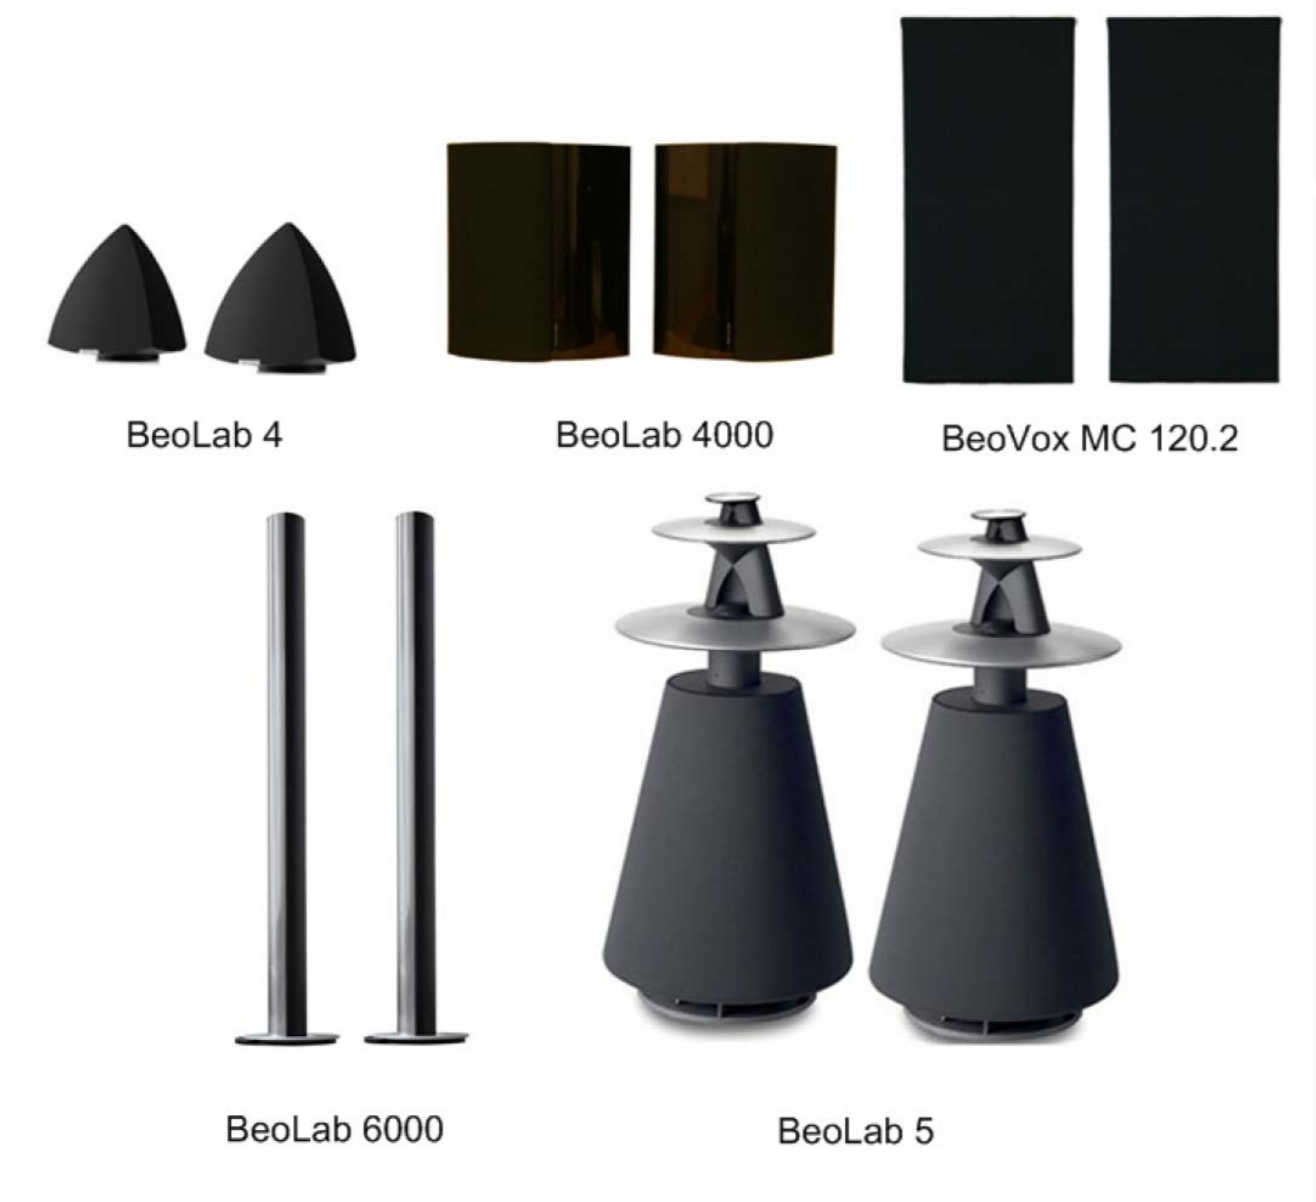
\includegraphics[scale = 0.7]{Figure/speakers.png}
\caption{A figure of the speakers used in the data set. They are all from Bang \& Olufsen in order to avoid any bias relating to specific brands}
\label{fig:speakers}
\end{figure}

The data is analyzed using the software \textit{PanelCheck}. The analysis is quite explorative, since it is still unknown what we are looking for. 